% Options for packages loaded elsewhere
\PassOptionsToPackage{unicode}{hyperref}
\PassOptionsToPackage{hyphens}{url}
%
\documentclass[
]{article}
\usepackage{amsmath,amssymb}
\usepackage{iftex}
\ifPDFTeX
  \usepackage[T1]{fontenc}
  \usepackage[utf8]{inputenc}
  \usepackage{textcomp} % provide euro and other symbols
\else % if luatex or xetex
  \usepackage{unicode-math} % this also loads fontspec
  \defaultfontfeatures{Scale=MatchLowercase}
  \defaultfontfeatures[\rmfamily]{Ligatures=TeX,Scale=1}
\fi
\usepackage{lmodern}
\ifPDFTeX\else
  % xetex/luatex font selection
\fi
% Use upquote if available, for straight quotes in verbatim environments
\IfFileExists{upquote.sty}{\usepackage{upquote}}{}
\IfFileExists{microtype.sty}{% use microtype if available
  \usepackage[]{microtype}
  \UseMicrotypeSet[protrusion]{basicmath} % disable protrusion for tt fonts
}{}
\makeatletter
\@ifundefined{KOMAClassName}{% if non-KOMA class
  \IfFileExists{parskip.sty}{%
    \usepackage{parskip}
  }{% else
    \setlength{\parindent}{0pt}
    \setlength{\parskip}{6pt plus 2pt minus 1pt}}
}{% if KOMA class
  \KOMAoptions{parskip=half}}
\makeatother
\usepackage{xcolor}
\usepackage{longtable,booktabs,array}
\usepackage{calc} % for calculating minipage widths
% Correct order of tables after \paragraph or \subparagraph
\usepackage{etoolbox}
\makeatletter
\patchcmd\longtable{\par}{\if@noskipsec\mbox{}\fi\par}{}{}
\makeatother
% Allow footnotes in longtable head/foot
\IfFileExists{footnotehyper.sty}{\usepackage{footnotehyper}}{\usepackage{footnote}}
\makesavenoteenv{longtable}
\usepackage{graphicx}
\makeatletter
\def\maxwidth{\ifdim\Gin@nat@width>\linewidth\linewidth\else\Gin@nat@width\fi}
\def\maxheight{\ifdim\Gin@nat@height>\textheight\textheight\else\Gin@nat@height\fi}
\makeatother
% Scale images if necessary, so that they will not overflow the page
% margins by default, and it is still possible to overwrite the defaults
% using explicit options in \includegraphics[width, height, ...]{}
\setkeys{Gin}{width=\maxwidth,height=\maxheight,keepaspectratio}
% Set default figure placement to htbp
\makeatletter
\def\fps@figure{htbp}
\makeatother
\usepackage{soul}
\setlength{\emergencystretch}{3em} % prevent overfull lines
\providecommand{\tightlist}{%
  \setlength{\itemsep}{0pt}\setlength{\parskip}{0pt}}
\setcounter{secnumdepth}{-\maxdimen} % remove section numbering
\ifLuaTeX
  \usepackage{selnolig}  % disable illegal ligatures
\fi
\IfFileExists{bookmark.sty}{\usepackage{bookmark}}{\usepackage{hyperref}}
\IfFileExists{xurl.sty}{\usepackage{xurl}}{} % add URL line breaks if available
\urlstyle{same}
\hypersetup{
  hidelinks,
  pdfcreator={LaTeX via pandoc}}

\author{}
\date{}

\begin{document}

\begin{longtable}[]{@{}l@{}}
\toprule\noalign{}
\endhead
\bottomrule\noalign{}
\endlastfoot
type: writing \\
status: active \\
priority: p1 \\
project: PENG9560 \\
creationtag: 2023-02-27 11:55 \\
infotags: \\
people: \\
date: \\
\end{longtable}

See {[}{[}PENG9560 Assignment Draft 1} See {[}{[}PENG9560
Assignment Draft 2} See {[}{[}PENG9560 Assignment Draft 3}

\textbf{Cleaning up for latex.}

\hypertarget{introduction}{%
\section{Introduction}\label{introduction}}

The approach Reinforcement Learning (RL) takes that of some ``agent'' in
an environment where it must optimize its actions based on evaluations
environment's state, in order to optimize for a reward. This has its
basis in real-world biological models of learning, borrowing from
studies of animal models where an animal is conditioned to actions in
the presence of environmental inputs to elicit a reward such as food.

Current RL methods utilize tabular methods, where an association of
\emph{state} and \emph{action} is mapped to \emph{reward} as a
state-action pair, or a \emph{Q-policy}, denoted: \(Q(S, A)\). These
policies are optimized by some \emph{Q-function}.

For a \emph{Q-Function}, there is internally is a~Q-table that contains
all the \emph{Q-policies}: mappings between the state of the environment
and the subsequent most likely course of action to result in reward.
This is represented in the table by a \emph{Q-value}. Given a state and
action, our Q-Function~will search into its Q-table the corresponding
value.

However, this approach suffers the \emph{curse of dimensionality}. In
regimes of increasingly larger environmental input and action space, the
policy space scales exponentially.

Additionally, this discrete policy method fails in more naturalistic
regimes where spaces have continuous non-discrete values, causing
discrete mappings to fail as even small differences between values can
result in wildly different outcomes.

The success of Deep Neural Networks (DNN) which are able to encode
high-dimensional data in the latent space of relatively condense network
structures and capable of continuous mappings, offers a potential
solution to the inherent weaknesses of RL. However, this combination of
machine learning methods, until relatively recently, had no clear path
forward. The key training method in traditional Artificial Neural
Networks (ANN), back-propagation-through-time, can not be implemented in
a Q-policy framework.

A precursor to the paper reviewed here, and a cornerstone of the Deep
Reinforcement Learning (DRL) field Mnih et al 2015
\autocite{mnihHumanlevelControlDeep2015}, developed a novel DRL
network, which implemented a new form of Q-Learning titled
\emph{experience replay}. Experience replay, inspired by neuroscientific
models of hippocampal memory replay
\autocite{bendorBiasingContentHippocampal2012}
\autocite{oneillPlayItAgain2010}, randomizes over batches of the data,
removing correlations through time in the episode sequence. This
provides the basis for their highly-successful implementation of RL in
an DNN, dubbed a \textbf{\emph{Deep Q-Network (DQN)}}.

As all the methods so far have their basis in biological models of
learning, there is a need to further develop models which mimic the
capabilities and mechanisms of the human brain. Recent work has gone
into developing Spiking Neural Networks (SNN), networks imitate the
spiking functions of biological neurons at the neuronal level.

SNNs lie at an oblique juncture with traditional ANNs as the mode of
communication at the neuron level is fundamentally different. They
eschew ANNs' static and continuous-valued activation for the binary and
highly time-dependent information passing of spikes, where spike rates
and timing are important
\autocite{tanStrategyBenchmarkConverting2020}. The exact nature
of spiking communication in the human brain is highly-complex and not a
solved problem by any means. Many plausible mechanisms have been
successfully utilized in SNN models over the years
\autocite{vigneronCriticalSurveySTDP2020}.

The swath of potential benefits offered by SNNs is the main motivator
behind their development. Neuromorphics, hardware designed specifically
around SNNs to exploit their low-power power properties, alone offers an
economic incentive to their development. SNNs naturally encode time
information and utilize low-powered event-driven processing, which may
further the possibilities in online and self-supervised RL models.

In this paper we review Liu et al.~2022 - \emph{``Human-Level Control
Through Directly Trained Deep Spiking \(Q\)-Networks''}, which provides
a complete and effective implementation of RL, DNN, and SNNs; By
expanding on the original DQN network
\autocite{mnihHumanlevelControlDeep2015} with a full SNN
implementation. Liu et al.~2022 is the first of its kind to implement a
full spiking network, whereas any previous SNN-DQN models relied on a
traditional ANN at a point in the process. This review will cover the
methods of Liu et al.~2022 and how they built on models post-Mnih et
al.~2015.

\hypertarget{methods}{%
\section{Methods}\label{methods}}

\hypertarget{mnih-et-al-2015--dqn}{%
\subsection{Mnih et al 2015 -DQN}\label{mnih-et-al-2015--dqn}}

The \emph{Deep Q-network (DQN)} architecture on which these models are
based upon comes from Minh et al.~2015
\autocite{mnihHumanlevelControlDeep2015}. In broad strokes, this
model implements RL in a deep learning regime by mapping the Q-policies
into the state of the network by training the hyperparameters to the
target network with a Q-learning algorithm. An image is used as the
observed environmental input, the resultant Q-values being interpreted
as the values on the output layer, with each output node corresponding
to some action.

The implementation of RL into a DNN model does not come easily. RL
disallows for use of back propagation through time, where in Q-learning,
policies can be dependent on the trajectory of actions taken over
multiple time steps.

The authors of Mnih et al.~2015 provide a solution to this in what they
introduce as \emph{experience replay}. This method is inspired by
biological modes of learning where episodes of action in memory are
replayed during sleep. Likewise, experience replay that randomizes over
the data, to remove correlations in the observation sequence and
smoothing over changes in the data distribution. This is done by storing
episodes of experience at each time step
\(e_{t}= (s_{t} , a_{t}, r_{t}, s_{t+1})\) in a buffer, then for some
time window, a training step is performed, where a sub-sample of
experiences are randomly selected and trained on with Q-learning. In
order to stay a tractable problem the training step is done at regular
interval windows along the full length of the experiment, e.g.~every
100,000 timesteps.

As a benchmark the DQN was tested with 49 games from the Atari 2600,
with a different network being trained for each game. For each games,
the image of the current screen, action state, and score (corresponding
to the reward) is available to the model.

\hypertarget{dqn---architecture}{%
\subsubsection{DQN - Architecture}\label{dqn---architecture}}

The DQN is an ANN composed of three initial convolutional layers
followed by two fully-connected layers. A schematic of the architecture
is illustrated in {[}fig 1.{]}

The input layer intakes an 84 x 84 x 4 game frames which have been
preprocessed into 84 x 84 pixel images, with the 4 most recent frames at
the experience time step \(t\) in the subsample being selected.

The first hidden layer convolves 32 filters of 8 x 8 with stride. The
second hidden layer convolves 64 filters of 4 x 4 with stride 2. The
third and final convolution layer convolves 64 filters of 3 x 3 with
stride 1. Each convolution layer is rectified by ReLUs before passing to
the next layer.

The next two layers are fully-connected layers, the first consists of
512 rectifier units, and the output layer is a fully connected layer
with a number of outputs corresponding to the number of valid actions in
the Atari games tested. This varied between 4 and 18 actions in the
games tested.

The resulting model was able to reach and surpass human level
performance, in 29 of the 49 games tested.

\begin{figure}
\centering
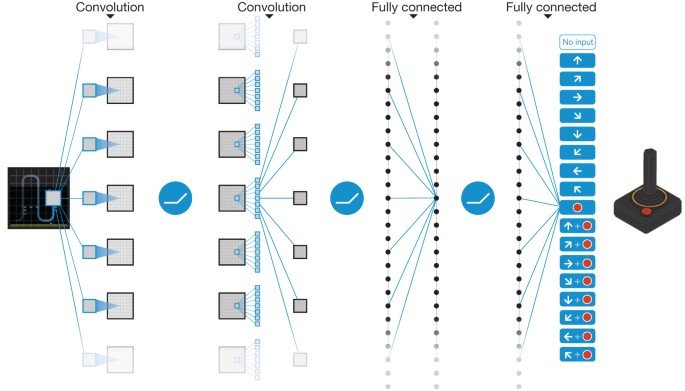
\includegraphics[width=0.7\textwidth,height=\textheight]{41586_2015_BFnature14236_Fig1_HTML.jpg}
\caption{\textbf{Fig. 1:} Adapted from
\autocite{mnihHumanlevelControlDeep2015}}
\end{figure}

\hypertarget{the-addition-of-an-snn}{%
\subsection{The addition of an SNN}\label{the-addition-of-an-snn}}

The goal of our Liu et al.~2022 is to take the well established
framework of \autocite{mnihHumanlevelControlDeep2015} and create a
full implementation of it with spiking neurons. The motivation for the
addition of spiking neurons is expanded on in
\autocite{zenkeVisualizingJointFuture2021}
\autocite{princeCurrentStateFuture2022}
\autocite{mehonicBraininspiredComputingNeeds2022} with the main
advantages being low-energy and low-computational costs. In RL they
potentially offer a powerful tool in designing fully-online and
self-supervising models.

The design of spiking neural networks is still relatively unexplored,
and our first steps are to implement these in established methods.
Likewise, as a biologically inspired model, there are potential benefits
from adaptation of neurological mechanisms in neural networks.
Neurological models, which are necessarily deep and reinforcement
trained, can possibly have their properties exploited for better DRL
models.

However, their unique and non-conventional communication technique means
implementation in traditional models requires some method of encoding
and decoding the spike activity.

Prior works which introduced SNNs to the DQN framework did so by
pre-training the ANN network before conversion into an SNN. This was
done by converting the ReLU units into \emph{Leaky Integrate and Fire
\textbf{(LIF)}} spiking units
\autocite{patelImprovedRobustnessReinforcement2019} and treating
the spike frequency over the training window as the output value. These
networks proved to perform similarly to the original DQN, and even
proved to be more robust to input perturbations than the DQN.

Tan et al.~2020 further improved the conversion of ANNs to SNNs, through
use of \emph{Integrate and Fire \textbf{(IF)}} neurons, which
approximates the ReLU output in its firing rate over time (explained
below). This improved the accuracy of the converted SNNs, and stands as
the example to which the authors of Liu et al 2022 compare their model
against. This model however still requires conversion from an ANN as
well as a larger simulation time window (100 time steps vs 64 in Liu et
al.~2022) making for a less tractable problem.

However, in order to train a full Deep SNN, there is an additional
caveat to mitigated. The spike function of the neuron is
non-differentiable, where the output is defined by the Heaviside step
function, and equal to 1 at the time of a spike, and equal to 0 at all
other times. This is mitigated by surrogate gradient descent, where the
Heaviside step-function is replace with a surrogate arctan function.

\hypertarget{liu-et-al.-2022---the-deep-spiking-q-network-dsqn}{%
\subsection{Liu et al.~2022 - The Deep Spiking Q-Network
(DSQN)}\label{liu-et-al.-2022---the-deep-spiking-q-network-dsqn}}

The Liu et al.~2022 model, which they title as the \emph{Deep Spiking
Q-Network \textbf{(DSQN)}}, replicates the Mnih et al.~2015 DQN
architecture, however with the full replacement of artificial units with
spiking LIF neurons. Thus, circumventing the need for a pretrained ANN
and obviating any issues arising during conversion between
architectures.

They describe the neuronal dynamics of the LIF neurons as follows, for
layer \(l \in\) \(\{1, \ldots, L-1\}\) at simulation time \(t\): \[
\begin{aligned}
U^{l, t} & =V^{l, t-1}+\frac{1}{\tau_{\mathrm{m}}}\left(W^l S^{l-1, t}-V^{l, t-1}+V_{\mathrm{r}}\right) \\
\end{aligned}
\] Equation (1) describes the pre-spike subthreshold membrane potential
of neurons. \(V_{\mathrm{th}}\) describes the threshold potential, the
limit at which if exceeded, the neuron will emit a spike and reset the
membrane voltage. \(\tau_{\mathrm{m}}\) denotes the membrane time
constant, essentially the decay rate at which membrane potential will
``leak.'' \(W^l\) denotes the learnable weights of the neurons in layer
\(l\), and \(V_{\mathrm{r}}\) denotes the initial membrane potential.

They describe two varieties of ``reset'' when the threshold membrane
voltage is exceeded, a ``hard reset'' which mimics the typical dynamics
of biological neurons, fully resetting the membrane potential back to
some baseline, typically \(V = 0\); and a ``soft reset'', a less common,
but still biologically plausible model of neuron dynamics, where after
exceeding the threshold, the threshold membrane potential is subtracted
from the current membrane potential. The membrane potential of neurons
when reached \(V_{\text {th }}\) is described by: \[
\begin{aligned}
V^{l, t} & = \begin{cases}U^{l, t}\left(1-S^{l, t}\right)+V_{\mathrm{r}} S^{l, t}, & \text { hard reset } \\
U^{l, t}-V_{\mathrm{th}} S^{l, t}, & \text { soft reset. }\end{cases}
\end{aligned}
\] Though for their experiments they only use the hard reset in LIF,
they exhibit this distinction to compare with previous methods which
rely on non-leaky IF neurons which was used for ANN to SNN conversions
as the IF neuron is reset by a soft reset as an unbiased estimator of
ReLU activation function over time (See {[}fig 2.{]} and {[}fig 3.{]}
for comparison).

!{[}\textbf{Fig.2:} Adapted from
\href{image-20230227160506589.png}{\autocite{liuHumanLevelControlDirectly2022}}

!{[}\textbf{Fig.3:} Adapted from
\href{image-20230227160709544.png}{\autocite{liuHumanLevelControlDirectly2022}}

They find that the LIF neuron with a hard reset to be more robust during
the training stage, with a wider range for different thresholds. ``LIF
neurons have more potential to obtain optimal results in our DSQN and
could be directly trained without relying on the normalization technique
in conversion methods''
\autocite{liuHumanLevelControlDirectly2022}.

The output of the LIF neurons in layer \(l \in\{1, \ldots, L-1\}\) at
simulation time \(t\) is described by the equation: \[
\begin{aligned}
S^{l, t} & =\Theta\left(U^{l, t}-V_{\text {th }}\right) \\
\Theta(x) & = \begin{cases}1, & x \geq 0 \\
0, & \text { otherwise }\end{cases}
\end{aligned}
\] where \(\Theta(x)\) is the spiking function of the neurons. As this
is a nondifferentiable function, a surrogate function must be used
during training. In this paper they use the arc-tangent function as it
provides less complexity in comparison to the sigmoid function, which is
also commonly used.

To read out the Q-values of the final layer, they take they sum of
weighted spike input from the final hidden layer over the time
simulation window. Their output is read as:
\[O^L=W^L \frac{1}{t} \sum_{t^{\prime}=1}^t S^{L-1, t^{\prime}}\]where
\(O^L\) denotes the output Q-values of DSQN, \(W^L\) is the learnable
weights of the neurons in the final layer, and t is the simulation time
window.

The DSQN is then trained according to the deep \(Q\)-learning algorithm
\autocite{mnihHumanlevelControlDeep2015}, using the following
loss function: \[
 \mathcal{L}(W)=\mathbb{E}_{\left(s, a, r, s^{\prime}\right) \sim U(D)}\left[\left(y_{\left(r, s^{\prime}\right)}-Q(s, a ; W)\right)^2\right]
 \] with \[
 y_{\left(r, s^{\prime}\right)}=r+\gamma \max _{a^{\prime}} Q\left(s^{\prime}, a^{\prime} ; W^{-}\right)
 \] where \(Q(s, a ; W)\) denotes the approximate \(Q\)-value function
parameterized by DSQN. \(W\) and \(W^{-}\)denote the weights of DSQN at
the current and previous steps, respectively.
\(\left(s, a, r, s^{\prime}\right) \sim\) \(U(D)\) denotes the
minibatches drawn uniformly at random from the experience replay memory
\(D\), and \(\gamma\) is the reward discount factor
\autocite{liuHumanLevelControlDirectly2022}.

\hypertarget{model-evaluation}{%
\section{Model Evaluation}\label{model-evaluation}}

The qualities measured for were, performance, stability, learning
capability, and energy efficiency. They compare their results against
their own reproductions of the original DQN model in Mnih et al.~2015 as
well as the conversion based SNN in Tan et al 2020. They used the 17 top
performing Atari games which were also used in Tan et al.~2020, these
are also the games for which the original DQN performed highest.

The in game frames are preprocessed to render them in greyscale and
down-resolutioned them into 84 x 84 pixel images. The \(m\) most recent
frames (where \(m=4\)) are stacked as input. The real pixel values are
fed as inputs to the network without neural encoding.

The game is then simulated with a training time step occurring with a
window of 64 time steps for the DSQN and 100 time steps for the
conversion based SNN.

In performance, of the 17 Atari games tested, the DSQN out-performed (in
terms of points) the DQN by an average of 106\%. The DSQN was able to
outperform the DQN on four games, scored equally in nine games, and
scored worst (maximum 20\% difference) in four of the games. Further, it
proved to be more stable, obtaining lower standard deviations in score
than the DQN in six games, equal to it on two games, and inferior in
nine games.

In learning capability, a total proof is not given. In {[}fig 4.{]} the
learning curve for the DQN and DSQN is compared for two games. From
these plots it is apparent that the DSQN reaches a higher score
equilibrium faster than the DQN, as well as in average max Q-value.
Though the authors claim this is representative in all cases, no metric
is provided. In the future an area under curve metric may be a useful
measure compare.

As with the DQN, we can see instability in the learning curves which is
native problem with the DQN. In DQNs this is mitigated through
implementation of a Double-DQN
\autocite{wengTianshouHighlyModularized2022} , where a
\emph{target network} is simultaneously trained to calculate the target
Q-values at the next state. The authors actually do implement this DQN
model as well as the more recent CDQN
\autocite{wangConvergentEfficientDeep2022}. The authors claim
their implementations of these variations claim a better performance to
their ANN counterparts by 151.4\% and 141.8\% to the Double-DQN and CDQN
respectively. Unfortunately, no standard deviation measurements are
provided, but comparison of {[}fig 4.{]} and {[}fig 5.{]} appears to
show less deviation.

Lastly, they score the model in terms of energy-efficiency. This is a
useful metric for prospective uses in neuromorphic hardware, where the
energy savings from spiking can be best obtained. However, there is no
direct method of comparing the DSQN to the DQN. A rough estimate can be
made by comparing the number of calculations needed per inference. In
terms of energy transfer, the SNN must be evaluated in average spike
count. In this case it was better to compare it to the conversion-based
SNN of \autocite{tanStrategyBenchmarkConverting2020}. The results show
the DSQN used around 85\% of the energy in comparison to the
conversion-based SNN. Though, this comparison was only shown for two
games.

!{[}\textbf{Fig.4:} Adapted from
\href{image-20230228103326947.png}{\autocite{liuHumanLevelControlDirectly2022}}

!{[}\textbf{Fig.5:} Adapted from
\href{image-20230228124237495.png}{\autocite{liuHumanLevelControlDirectly2022}}

\hypertarget{review}{%
\section{Review}\label{review}}

I find Liu et al.~2022 to be a very thorough and complete work which
takes the next logical step in deep reinforcement learning networks with
spiking neurons. This paper appears to be the first to showcase DRL in a
fully SNN model, where as other models require conversion of pre-trained
ANNs, or mediatory ANN side-networks
\autocite{chenDeepReinforcementLearning2022}. The following
proof of increased performance and robustness with a full SNN model,
sets the stage for future models designed around total SNN architecture.

The paper is a very exhaustive with fine detail of network architecture,
neuron design, training methods, as well as thorough comparison with a
breadth of other models in the experiments. The provided methods and
code repositories makes readily the reproduction of their model. Though
as of writing, the original github repository is unavailable.

As with Mnih et al.~2015, this paper will likely serve as milestone
against which to benchmark future DSRL models. The success of a fully
spiking model in this example means development of larger models which
utilize SNN's efficiency to address problems with larger state and
action spaces.

Additionally, there are mechanisms here that future Deep SNN learning
methods may be expected to duplicate. Namely, experience-replay, which
is again based on biological processes of memory formation and learning.
\autocite{mnihHumanlevelControlDeep2015} directly based the concept on
hippocampal replay wherein the during sleep, the brain replays
time-condensed activation of neural circuits associated with an
experienced physical activity
\autocite{bendorBiasingContentHippocampal2012}\autocite{oneillPlayItAgain2010}.
In SNNs, where spike timing larger oscillatory time cycles of neuron
activity known as phases are critical to network communication, perhaps
a designed neuronal circuit based around replicating the buffer like
memory and replaying the buffer in phases of time could be an aim of
future experiments.

Because the varieties of spiking neurons has no canonical set, further
experiments may be done with variations in neuron types, as well as
unique training methods specific to them. Testing their performance in a
DSQN will provide a valuable benchmark.

However, the reliance on gradient training may prove to be a
computational bottleneck. It may be prudent to then test the capacity
and computational costs of DSQNs. The unique properties of SNN
communication may prove the development of alternate training techniques
to better suit an accelerate their performance.

\hypertarget{further-directions}{%
\section{Further Directions}\label{further-directions}}

While this paper marks an important milestone in the development of deep
spiking reward based models, its efficacy in a naturalistic environment
that the typical biological agent may find itself in, is extremely
limited. The experience-replay method effectively leverages a Q-learning
framework to work in a DNN, but this limits the DSQN model to an offline
training algorithm for an offline, single-task-specific network.

While not the totality of RL motivations, a reward based framework can
allow for a dynamically adapting model able to train in an online and
self-supervised environment. With the goal in mind of designing
autonomous and reactive hardware, there is a need for models which are
able to learn and adapt to unpredictable and isolated environments. The
DSQN can inform us of the capabilities of an in-place SNN trained with
an RL framework. The next step is experiment with reward mechanisms
which will allow for dynamic learning in an online setting. To this
purpose it is necessary to replicate the abilities of SNNs similar to
those found in biological agents.

To this we are studying biologically inspired processes of credit
assignment. Local plasticity is a well known mechanism of adaptation at
the neuron and neuronal assembly level. A well studied mechanism that is
being studied for use in SNNs is that of Spike-Timing Dependent
Plasticity (STDP) as well as its extension \emph{three-factor dependent
plasticity} which performs training updates on the basis of a
\emph{third-factor} which may come in the form of a reward-signal.
Additionally, proposed methods of back-propagation in SNNs have lately
been proposed \autocite{payeurBurstdependentSynapticPlasticity2021}
\autocite{williamsNeuralBurstCodes2021} further adding alternative
plausible methods of credit-assignment in Deep-SNNs.

This however is a fairly nascent field, while emerging over two decades
ago in 1996 \autocite{maassNetworksSpikingNeurons1997}, it has gained
heavy traction in the past few years
\autocite{princeCurrentStateFuture2022}
\autocite{mehonicBraininspiredComputingNeeds2022} alongside
accelerating computational neuroscience and application specific
integrated circuits in the machine learning space; And so there is need
to develop and test the efficacy of proposed methods in this space.

At this point we are approaching a model of reinforcement learning from
an entirely new direction. This can be considered as a gap between
artificially driven methods and biologically-inspired ones, and there is
recent motivation to bridge the field of neuroscience back to deep
learning \autocite{zenkeVisualizingJointFuture2021} , by designing
entirely new mechanisms of reward-based learning that are effective in
SNNs, as opposed to attempting to apply the methods designed for ANNs,
then somewhat awkwardly fitting SNNs to them. This is not to say the
gains made from the ANN-to-SNN approach are non-contributive, but
instead we can use these proven models such as the DSQN to bridge the
gap from one direction, and build towards it from the other. Any future
Deep SNN implementations will need to match the benchmark set here by
Liu et al.~2022.

\hypertarget{references}{%
\section{References}\label{references}}

\autocite{chenDeepReinforcementLearning2022}

\autocite{mnihHumanlevelControlDeep2015}

\autocite{wangDeepReinforcementLearning2022}

\autocite{liuHumanLevelControlDirectly2022} - uh this looks similar if
not basically the same

\autocite{tanStrategyBenchmarkConverting2020} - an earlier paper which
does similar - referenced in both papers - In Liu they refer to this as
``conversion-based SNN'' - the compare their results in Liu to both Mnih
and this one - I don't think I want to linger on this as, from the sound
of it, it is pretrained on ANNs which are then converted to SNNs -
\st{They also have a DSQN CV} - They do not, I confused the subititle on
table VI in Liu - It is the comparison \textgreater{} - To further
improve the performance, Tan et al.~{[}28{]} proposed a more effective
conversion method based on the more accurate approximation of the
spiking firing rates. It reduced the conversion error based on a
pretrained DQN, and achieved state-of-the-art performance on multiple
Atari games.

{[}24{]} D. Patel, H. Hazan, D. J. Saunders, H. T. Siegelmann, and R.
Kozma, ``Improved robustness of reinforcement learning policies upon
conversion to spiking neuronal network platforms applied to atari
breakout game,'' Neural Networks, vol.~120, pp.~108--115, 2019.
\autocite{patelImprovedRobustnessReinforcement2019}

\begin{quote}
is the first work to introduce spiking conversion methods to the domain
of deep Q-learning. They demonstrated that both shallow and deep ReLU
networks can be converted to SNNs without performance degradation on
Atari game Breakout. Then, they showed that the converted SNN is more
robust to input perturbations than the original neural network. However,
it only focuses on improving the robustness rather than the performance
of SNNs on Atari games.
\end{quote}

{[}26{]} B. Rueckauer, I.-A. Lungu, Y. Hu, M. Pfeiffer, and S.-C. Liu,
``Conversion of continuous-valued deep networks to efficient eventdriven
networks for image classification,'' Front. Neurosci., vol.~11, p.~682,
Dec.~2017. \autocite{rueckauerConversionContinuousValuedDeep2017}

{[}44{]} J. Weng et al., ``Tianshou: A highly modularized deep
reinforcement learning library,'' 2021, arXiv:2107.14171.
\autocite{wengTianshouHighl|yModularized2022}

{[}45{]} Z. T. Wang and M. Ueda, ``Convergent and efficient deep Q
learning algorithm,'' in Proc. Int. Conf. Learn. Represent., Mar.~2022,
pp.~1--27. \autocite{wangConvergentEfficientDeep2022}

\autocite{zenkeVisualizingJointFuture2021}
\autocite{princeCurrentStateFuture2022}
\autocite{mehonicBraininspiredComputingNeeds2022}

\end{document}
